% Author: Dun-Ming Huang
% Email: dunmingbrandonhuang@berkeley.edu
% CSM16A Fall 2022

\begin{center}
    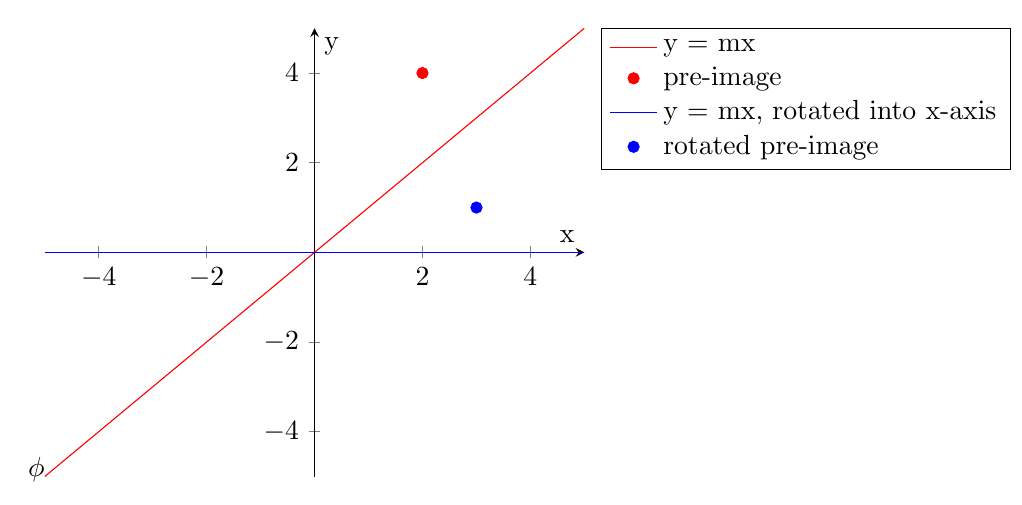
\begin{tikzpicture}
        \tkzDefPoint(3.5,2.8){O}
        \tkzDefPoint(6.5,5.8){A}
        \tkzDefPoint(6.5,2.8){B}
        \tkzMarkAngle[line width = 1.5pt, arrows = <-](B,O,A)
        \tkzLabelAngle[pos=1.5](B,O,A){$\phi$}
        \begin{axis}[
            axis lines = middle,
            xmin=-5, xmax=5,
            ymin=-5, ymax=5,
            xlabel = {x},
            ylabel = {y},
            legend pos=outer north east,
            legend cell align=left
        ]
            \addplot [color=red] {
               x
            };
            \addlegendentry{y = mx}
            \addplot [only marks, color=red] table {
                2 4
            };
            \addlegendentry{pre-image}
            \addplot [color=blue] {
               0
            };
            \addlegendentry{y = mx, rotated into x-axis}
            \addplot [only marks, color=blue] table {
                3 1
            };
            \addlegendentry{rotated pre-image}
        \end{axis}
    \end{tikzpicture}
\end{center}